\documentclass{beamer}
\usepackage{tikz}
\usepackage{graphicx}
\usepackage{subcaption}
\usepackage{pgfplots}
\pgfplotsset{compat=1.17}


\begin{document}

\frame{\frametitle{\textbf{Bag of Words}}
\framesubtitle{\textbf{Definition, Vectorization, Advantages and Disadvantages}}

\begin{itemize}
  \item \textbf{Bag of Words (BoW)} represents a document as a collection of its constituent words, ignoring grammar and word order.
  \item {Example}:
  \begin{itemize}
    \item Sentence 1: "The cat sat on the mat near another cat."
    \item Sentence 2: "The dog jumped over the fence."
  \end{itemize}
\end{itemize}

\begin{center}
\begin{tabular}{|c|c|c|c|c|c|c|}
  \hline
  & \textbf{cat} & \textbf{dog} & \textbf{fence} & \textbf{jumped} & \textbf{mat} & \textbf{sat} \\
  \hline
  \textbf{Sentence 1} & 2 & 0 & 0 & 0 & 1 & 1 \\
  \hline
  \textbf{Sentence 2} & 0 & 1 & 1 & 1 & 0 & 0 \\
  \hline
\end{tabular}
\end{center}

\begin{itemize}
  \item \textbf{Advantages}:
  \begin{itemize}
    \item Simple and easy to implement.
    \item Preserves the semantic meaning of words in the document.
  \end{itemize}
  \item \textbf{Disadvantages}:
  \begin{itemize}
    \item Ignores grammar and word order, resulting in loss of contextual information.
    \item Increases dimensionality and sparsity of the vector representation.
  \end{itemize}
\end{itemize}

}

\frame{\frametitle{\textbf{Sac de Mots (Bag of Words)}}
\framesubtitle{\textbf{Définition, Vectorisation, Avantages et Inconvénients}}


\begin{itemize}
  \item \textbf{Sac de Mots (BoW)} représente un document comme une collection de ses mots constitutifs, ignorant la grammaire et l'ordre des mots.
  \item {Exemple}:
  \begin{itemize}
    \item Phrase 1: "Le chat dort sur le chat."
    \item Phrase 2: "Le chien saute."
  \end{itemize}
\end{itemize}

\begin{center}
\begin{tabular}{|c|c|c|c|c|}
  \hline
  & \textbf{chat} & \textbf{chien} & \textbf{dort} & \textbf{saute} \\
  \hline
  \textbf{Phrase 1} & 2 & 0 & 1 & 0 \\
  \hline
  \textbf{Phrase 2} & 0 & 1 & 0 & 1 \\
  \hline
\end{tabular}
\end{center}

\begin{itemize}
  \item \textbf{Avantages}:
  \begin{itemize}
    \item Simple et facile à implémenter.
    \item Préserve la signification sémantique des mots dans le document.
  \end{itemize}
  \item \textbf{Inconvénients}:
  \begin{itemize}
    \item Ignore la grammaire et l'ordre des mots, entraînant une perte d'informations contextuelles.
    \item Augmente la dimensionnalité et la parcimonie de la représentation vectorielle.
  \end{itemize}
\end{itemize}

}



\frame{\frametitle{K-Nearest Neighbors (KNN)}
\framesubtitle{Advantages, Disadvantages, and Illustration}

\textbf{Advantages:}
\begin{itemize}
  \item Simple and easy to implement.
  \item Non-parametric method.
  \item Suitable for both classification and regression tasks.
\end{itemize}

\textbf{Disadvantages:}
\begin{itemize}
  \item Computationally expensive for large datasets.
  \item Sensitive to the choice of k and distance metric.
  \item Performs poorly with high-dimensional data.
\end{itemize}

\begin{center}
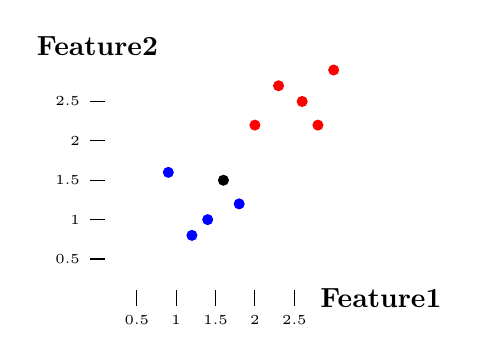
\begin{tikzpicture}
    % Blue points
    \foreach \point in {(1.2,0.8), (1.8,1.2), (0.9,1.6), (1.4,1)} {
        \fill[blue] \point circle (2pt);
    }
    
    % Red points
    \foreach \point in {(2,2.2), (2.6,2.5), (2.3,2.7), (3,2.9), (2.8,2.2)} {
        \fill[red] \point circle (2pt);
    }

    % Black point (test subject)
    \fill[black] (1.6,1.5) circle (2pt);
    
    % Axis labels
    \node at (3.6,0) {{\textbf{Feature1}}};
    \node at (0,3.2) {{\textbf{Feature2}}};
    
    % Axis ticks
    \draw (0.5,0.1) -- (0.5,-0.1) node[below] {\tiny{0.5}};
    \draw (1,0.1) -- (1,-0.1) node[below] {\tiny{1}};
    \draw (1.5,0.1) -- (1.5,-0.1) node[below] {\tiny{1.5}};
    \draw (2,0.1) -- (2,-0.1) node[below] {\tiny{2}};
    \draw (2.5,0.1) -- (2.5,-0.1) node[below] {\tiny{2.5}};
    
    \draw (0.1,0.5) -- (-0.1,0.5) node[left] {\tiny{0.5}};
    \draw (0.1,1) -- (-0.1,1) node[left] {\tiny{1}};
    \draw (0.1,1.5) -- (-0.1,1.5) node[left] {\tiny{1.5}};
    \draw (0.1,2) -- (-0.1,2) node[left] {\tiny{2}};
    \draw (0.1,2.5) -- (-0.1,2.5) node[left] {\tiny{2.5}};
\end{tikzpicture}
\end{center}
}

\frame{\frametitle{K-Plus Proches Voisins (KPP ou KNN)}
\framesubtitle{Avantages, Inconvénients et Illustration}

\textbf{Avantages :}
\begin{itemize}
  \item Simple et facile à implémenter.
  \item Méthode non paramétrique.
  \item Convient à la fois pour les tâches de classification et de régression.
\end{itemize}

\textbf{Inconvénients :}
\begin{itemize}
  \item Coûteux en calcul pour les grands ensembles de données.
  \item Sensible au choix de k et de la métrique de distance.
  \item Performances médiocres avec des données de grande dimension.
\end{itemize}

\begin{center}
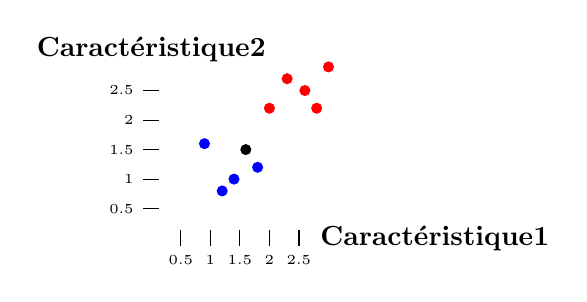
\begin{tikzpicture}
    % Points bleus
    \foreach \point in {(0.9,0.6), (1.35,0.9), (0.675,1.2), (1.05,0.75)} {
        \fill[blue] \point circle (2pt);
    }
    
    % Points rouges
    \foreach \point in {(1.5,1.65), (1.95,1.875), (1.725,2.025), (2.25,2.175), (2.1,1.65)} {
        \fill[red] \point circle (2pt);
    }

    % Point noir (sujet test)
    \fill[black] (1.2,1.125) circle (2pt);
    
    % Étiquettes des axes
    \node at (3.6,0) {{\textbf{Caractéristique1}}};
    \node at (0,2.4) {{\textbf{Caractéristique2}}};
    
    % Graduations des axes
    \draw (0.375,0.1) -- (0.375,-0.1) node[below] {\tiny{0.5}};
    \draw (0.75,0.1) -- (0.75,-0.1) node[below] {\tiny{1}};
    \draw (1.125,0.1) -- (1.125,-0.1) node[below] {\tiny{1.5}};
    \draw (1.5,0.1) -- (1.5,-0.1) node[below] {\tiny{2}};
    \draw (1.875,0.1) -- (1.875,-0.1) node[below] {\tiny{2.5}};
    
    \draw (0.1,0.375) -- (-0.1,0.375) node[left] {\tiny{0.5}};
    \draw (0.1,0.75) -- (-0.1,0.75) node[left] {\tiny{1}};
    \draw (0.1,1.125) -- (-0.1,1.125) node[left] {\tiny{1.5}};
    \draw (0.1,1.5) -- (-0.1,1.5) node[left] {\tiny{2}};
    \draw (0.1,1.875) -- (-0.1,1.875) node[left] {\tiny{2.5}};
\end{tikzpicture}
\end{center}
}



\begin{frame}{KNN Analysis (1)}
    
\begin{figure}[h]
    \centering
    \includegraphics[width=0.4\textwidth]{balancek5.png}
    \hspace{0.5cm}
    \includegraphics[width=0.4\textwidth]{balancek50.png}
    \vspace{0.5cm}
    \includegraphics[width=0.4\textwidth]{balancek500.png}
    \caption{Positive comments are labeled as true and negative comments are labeled as false for different values of k}
    \label{fig:balancenk}
\end{figure}

\end{frame}


\begin{frame}
\frametitle{KNN Analysis (2)}

\begin{figure}[h]
  \centering
  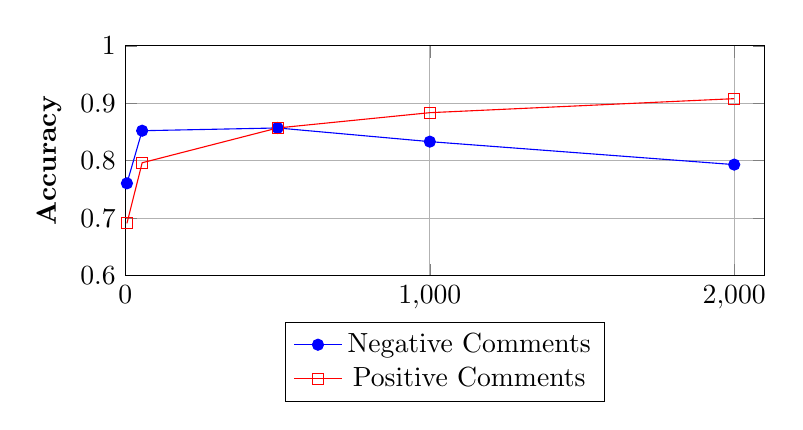
\begin{tikzpicture}
      \begin{axis}[
          xlabel={\textbf{k}},
          ylabel={\textbf{Accuracy}},
          xmin=0, xmax=2100,
          ymin=0.6, ymax=1,
          xtick={0,1000,2000,3000,4000,5000},
          ytick={0.6,0.7,0.8,0.9,1},
          legend style={at={(0.5,-0.2)}, anchor=north},
          grid=both,
          grid style={line width=0.2pt, draw=gray!30},
          major grid style={line width=0.4pt,draw=gray!60},
          height=4.5cm,
          width=0.8\textwidth
      ]
      \addplot[color=blue, mark=*] coordinates {
          (5,0.7606)
          (55,0.8522)
          (500,0.857)
          (1000,0.8332)
          (2000,0.7932)
      };
      \addplot[color=red, mark=square] coordinates {
          (5,0.691)
          (55,0.7964)
          (500,0.857)
          (1000,0.8836)
          (2000,0.908)
      };
      \legend{Negative Comments, Positive Comments}
      \end{axis}
  \end{tikzpicture}
  \caption{k nearest neighbor on balanced data}
  \label{fig:KNN1}
\end{figure}

\vspace{-0.8cm} % Adjust vertical space here

\begin{table}[h]
  \centering
  \begin{tabular}{@{}ccccc@{}}
  \hline
  Class & Precision & Recall & F1-Score & Support \\
  \hline
  False (negative comments) & 0.23 & 0.91 & 0.37 & 1789 \\
  True (positive comments) & 0.99 & 0.76 & 0.86 & 22520 \\
  \hline
  \multicolumn{5}{c}{Accuracy = 0.77} \\
  \hline
  \end{tabular}
  \caption{Classification report with undersampling}
  \label{tab:KNN}
\end{table}

\end{frame}

\begin{frame}
\frametitle{KNN Analysis with Different Options}

\begin{figure}[h]
  \centering
  \begin{tabular}{|c|c|c|c|}
  \hline
  & \textbf{BoW} & \textbf{tf-idf} & \textbf{One-hot} \\ \hline
  \textbf{Euclidean} & 0.7642 (1) & 0.7425 (113) & 0.6864 (5) \\ \hline
  \textbf{Cosine} &  0.7725 (1) & 0.7771 (1) & 0.6864 (5) \\ \hline
  \end{tabular}
  \caption{Comparative Accuracy Results, (k)}
  \label{tab:accuracy}
\end{figure}

\vspace{-0.5cm} % Adjust vertical space here

\begin{figure}[h]
  \centering
  \includegraphics[width=7cm]{accuracy_plot.png}
  \vspace{-0.2cm} % Adjust vertical space here
  \caption{Variation of accuracy with k (KNN, euclidean distance, BoW)}
  \label{fig:KNNOptions}
\end{figure}

\end{frame}

\begin{frame}
\frametitle{Insights - Analysis}

\begin{columns}

\begin{column}{0.6\textwidth}
\textbf{Challenges encountered:}
\begin{itemize}
\item Handling large dataset
\item Decisions on preprocessing
\end{itemize}

\textbf{Lessons learned:}
\begin{itemize}
\item Preprocessing is critical
\item Importance of class imbalance handling
\end{itemize}

\textbf{Limitations and Improvements:}
\begin{itemize}
\item Dealing with subjective sentiments
\item Domain adaptation challenges
\item Exploration of Deep Learning models
\end{itemize}

\end{column}

\begin{column}{0.5\textwidth}
\includegraphics[width=1\textwidth]{ezgif.com-gif-maker.png}
\end{column}

\end{columns}

\end{frame}

\begin{frame}
\frametitle{Analyse - Conclusions}

\begin{columns}

\begin{column}{0.6\textwidth}
\textbf{Défis rencontrés :}
\begin{itemize}
\item Gérer un grand jeu de données
\item Décisions sur le prétraitement
\end{itemize}

\textbf{Leçons apprises :}
\begin{itemize}
\item Le prétraitement est crucial
\item Importance de la gestion du déséquilibre des classes
\end{itemize}

\textbf{Limitations et améliorations :}
\begin{itemize}
\item Gérer les sentiments subjectifs
\item Défis de l'adaptation au domaine
\item Exploration de modèles de Deep Learning
\end{itemize}

\end{column}

\begin{column}{0.5\textwidth}
\includegraphics[width=1\textwidth]{img_neural_networks.jpg}
\end{column}

\end{columns}

\end{frame}


\end{document}


